\chapter{Scoping}\label{ch:scoping}

- [X] introduzione
- [X] chi siamo
- [X] chi sono i committenti
- [X] richiesta del cliente
  - [X] i loro problemi che vogliono risolvere
- [ ] analisi del dominio (meeting fatti)
  - [ ] event storming
- [ ] user stories  
- [ ] POS 


\section{Profilo della software house}\label{sec:profilo-della-software-house}
Atedeg è una software house che opera sul territorio cesenate. È composta da un team piuttosto affiatato di 10 persone dalle competenze più variegate, che si occupano di sviluppo software.

Il core team è composto da Giacomo, Linda, Nicolas e Nicolò, quattro amici che si sono conosciuti all'università e hanno deciso, una volta terminati gli studi, di fondare la software house.
Nel corso degli anni, il team si è arricchito di nuovi membri, che hanno portato con sé nuove idee e hanno contribuito a mantenere Atedeg un ambiente dinamico aperto all'innovazione. 

Essendo una piccola software house, Atedeg non adotta una rigida suddivisione gerarchica dei ruoli. In particolare, non esiste un senior management che decida quali progetti intraprendere o meno: infatti, tali decisioni vengono prese in comune dai membri del team, che si riuniscono periodicamente per discutere di nuovi possibili progetti. In questo modo, tutti i colleghi hanno la possibilità di esprimere le proprie opinioni e di partecipare attivamente alla vita dell'azienda.

All'interno di Atedeg si dà molta importanza all'arricchimento personale e professionale, e si cerca di dare a tutti gli sviluppatori la possibilità di crescere e di migliorare le proprie competenze. Per questo motivo sono incentivati lo studio e la formazione e, qualora i dipendenti ne facciano richiesta, l'azienda cerca di finanziare la loro partecipazione a conferenze di calibro internazionale. \todo[inline]{Mettere nella organizzazione delle ore il fatto che uno dei membri deve andare a una conferenza a Zurigo per tre giorni} In particolare, Linda ha avuto modo di assistere al ciclo di conferenze \href{https://dddeurope.com}{\emph{Domain Driven Design Europe}} del 2019 e da quel momento ha cercato di introdurre gradualmente nell'azienda il Domain Driven Design, che è stato adottato in due progetti conclusi con successo.

\section{Profilo del committente}\label{sec:profilo-del-committente}
Mambelli è un caseificio di Cesena a gestione familiare che si occupa di produzione e vendita di prodotti caseari. L'azienda è stata fondata nel 1972 e nel corso degli anni si è arricchita di nuove produzioni ricevendo anche diversi riconoscimenti come il premio \emph{Italian Cheese Award}. 
Grazie alla crescente popolarità è aumentata anche la domanda di prodotti e, per poterla soddisfare, Mambelli ha deciso di migliorare il proprio sistema informativo automatizzando i diversi processi aziendali laddove possibile.

L'azienda è gestita da Raffaella che si occupa dell'acquisto delle materie prime e della pianificazione della produzione dei formaggi. Il marito di Raffaella, Gianluca, si occupa invece dei rapporti coi clienti e della gestione degli ordini. Inoltre il caseificio assume due casari che si occupano della produzione dei formaggi e del controllo qualità dei prodotti. Infine l'azienda ha diversi dipendenti impiegati nel settore della logistica.

\section{Richiesta del committente}\label{sec:richiesta-del-committente}
L'attuale sistema informativo adottato dal caseificio Mambelli risulta inadeguato per poter gestire l'aumento nella domanda dei prodotti: molti dei processi aziendali sono infatti gestiti manualmente o su semplici fogli elettronici. In particolare, i problemi che il caseificio vorrebbe risolvere sono i seguenti:
\begin{itemize}
  \item \textbf{Gestione degli ordini:} al momento tutti gli ordini arrivano tramite mail o, in maniera informale, tramite comunicazioni telefoniche. Gianluca impiega quindi molto tempo per raccoglierli e inserirli nel sistema informativo. Inoltre, non essendo strutturati, gli ordini non sono facilmente consultabili e non è possibile ricavare informazioni utili per la pianificazione della produzione
  \item \textbf{Pianificazione della produzione:} la pianificazione di quali prodotti mandare in produzione viene fatta manualmente da Raffaella sulla base della sua grande esperienza nel campo. Per prendere queste decisioni Raffaella consulta un foglio elettronico che riporta alcune informazioni sugli ordini passati e su quanto è stato prodotto in precedenza. Sebbene questo metodo sia sufficiente per poter effettuare la programmazione, presenta due importanti problemi:
  \begin{itemize}
    \item Raffaella, grazie alla sua esperienza, è l'unica in grado di pianificare la produzione; se dovesse essere assente per qualche motivo, la produzione non potrebbe essere pianificata in maniera adeguata
    \item Sebbene l'esperienza di Raffaella sia sufficiente per avere delle buone pianificazioni, queste potrebbero essere ottimizzate ulteriormente con il supporto di sistemi informativi più avanzati riducendo i tempi morti nell'uso dei macchinari e minimizzando gli sprechi di materie prime
  \end{itemize}
  \item \textbf{Integrazione con sistemi preesistenti:} il caseificio Mambelli utilizza altri moduli software per gestire la tracciabilità dei prodotti e lo stoccaggio delle merci; per questo motivo è fondamentale che qualunque sistema realizzato possa essere integrato con questi sistemi
\end{itemize}
\todo[inline]{Far vedere che ci sono state le lezioncine di aggiornamento e che hanno portato a un leggero ritardo nella prima settimana}
\todo[inline]{Far vedere che nelle riunioni emergono ulteriori pain point: integrazione col sistema della tracciabilità, etc.}
\todo[inline]{Possibile rischio è che i clienti non apprezzino il nuovo sistema per gli ordini, mitigazioni che possiamo adottare: 
User Experience e incontri con persone per farglielo provare, suggerimento all'azienda di mettere sconti inizialmente per chi fa gli ordini online, NLP che estrae dalla mail il contenuto dell'ordine (questo però introduce ulteriori rischi)}

\section{Project Scoping Meeting}
\label{sec:project-scoping-meeting}

Il team di Atedeg ha valutato se prendere in considerazione o meno la proposta fatta dal caseificio. Dalla descrizione dei bisogni del committente riportata alla sezione precedente, emerge come il dominio del problema sia piuttosto ampio: infatti sarebbe richiesta la realizzazione di un sistema per la gestione degli ordini dei clienti che si possa integrare con altri sistemi eventualmente adottati. Inoltre, il secondo punto delle richieste potrebbe necessitare la realizzazione di un sistema di supporto alle decisioni con una profonda conoscenza del dominio del caseificio.
Linda propone quindi di effettuare una prima riunione con il committente per discutere la proposta adottando una metodologia improntata sul Domain Driven Design; infatti, questo approccio risulta ideale per domini aziendali simili ed è già stato utilizzato con successo dal team.

\todo[inline]{Descrizione generale dell'andamento dei meeting}


\subsection{Prima riunione}
\label{sec:prima-riunione}
Lo scopo della prima riunione è stato quello di discutere la proposta del committente e permettere al core team del progetto di conoscere il dominio del caseificio. Il committente ha messo a disposizione la propria sala riunioni per tre ore per svolgere il primo incontro. 
Su suggerimento di Linda, si è deciso di adottare la tecnica dell'\emph{Event Storming}~\cite{cit:event-storming} per condurre la riunione. 


\subsubsection{Setup della riunione}
\label{sec:setup-della-riunione}
Sebbene il committente abbia fornito la sala riunioni per tutta la mattinata (dalle 9:00 alle 12:00) il team ha segnato le 9:30 come orario di inizio effettivo per avere il tempo di preparare in maniera opportuna la sala.
Infatti, questa presenta la classica disposizione con un grande tavolo al centro circondato da sedie. Secondo Brandolini, padre dell'Event Storming, questo è un ``anti pattern'': infatti, porta i partecipanti a pensare che il meeting si svolgerà come tutte le altre (noiose) riunioni aziendali dove una persona parla e gli altri stanno seduti ad ascoltare~\cite[pp.~116-118]{cit:event-storming-book}.

L'approccio dell'Event Storming vuole puntare su una forte interazione fra i diversi esperti dei settori aziendali per approfondire la conoscenza del dominio e allo stesso tempo far emergere i veri bisogni del cliente. Per ottenere questo risultato si organizza la riunione in modo da sorprendere i partecipanti incentivandoli a una partecipazione attiva.

Quindi è stato appeso un grande rotolo di carta lungo tutta una parete della sala e sono stati messi a disposizione numerosi blocchetti di post-it colorati e pennarelli come mostrato in \Cref{fig:event-storming-setup}. Inoltre, il grande tavolo è stato spostato dal centro della stanza e le sedie sono state impilate per scoraggiare che i partecipanti si siedano durante la riunione diventando degli osservatori passivi.

\begin{figure}[!ht]
  \centering
  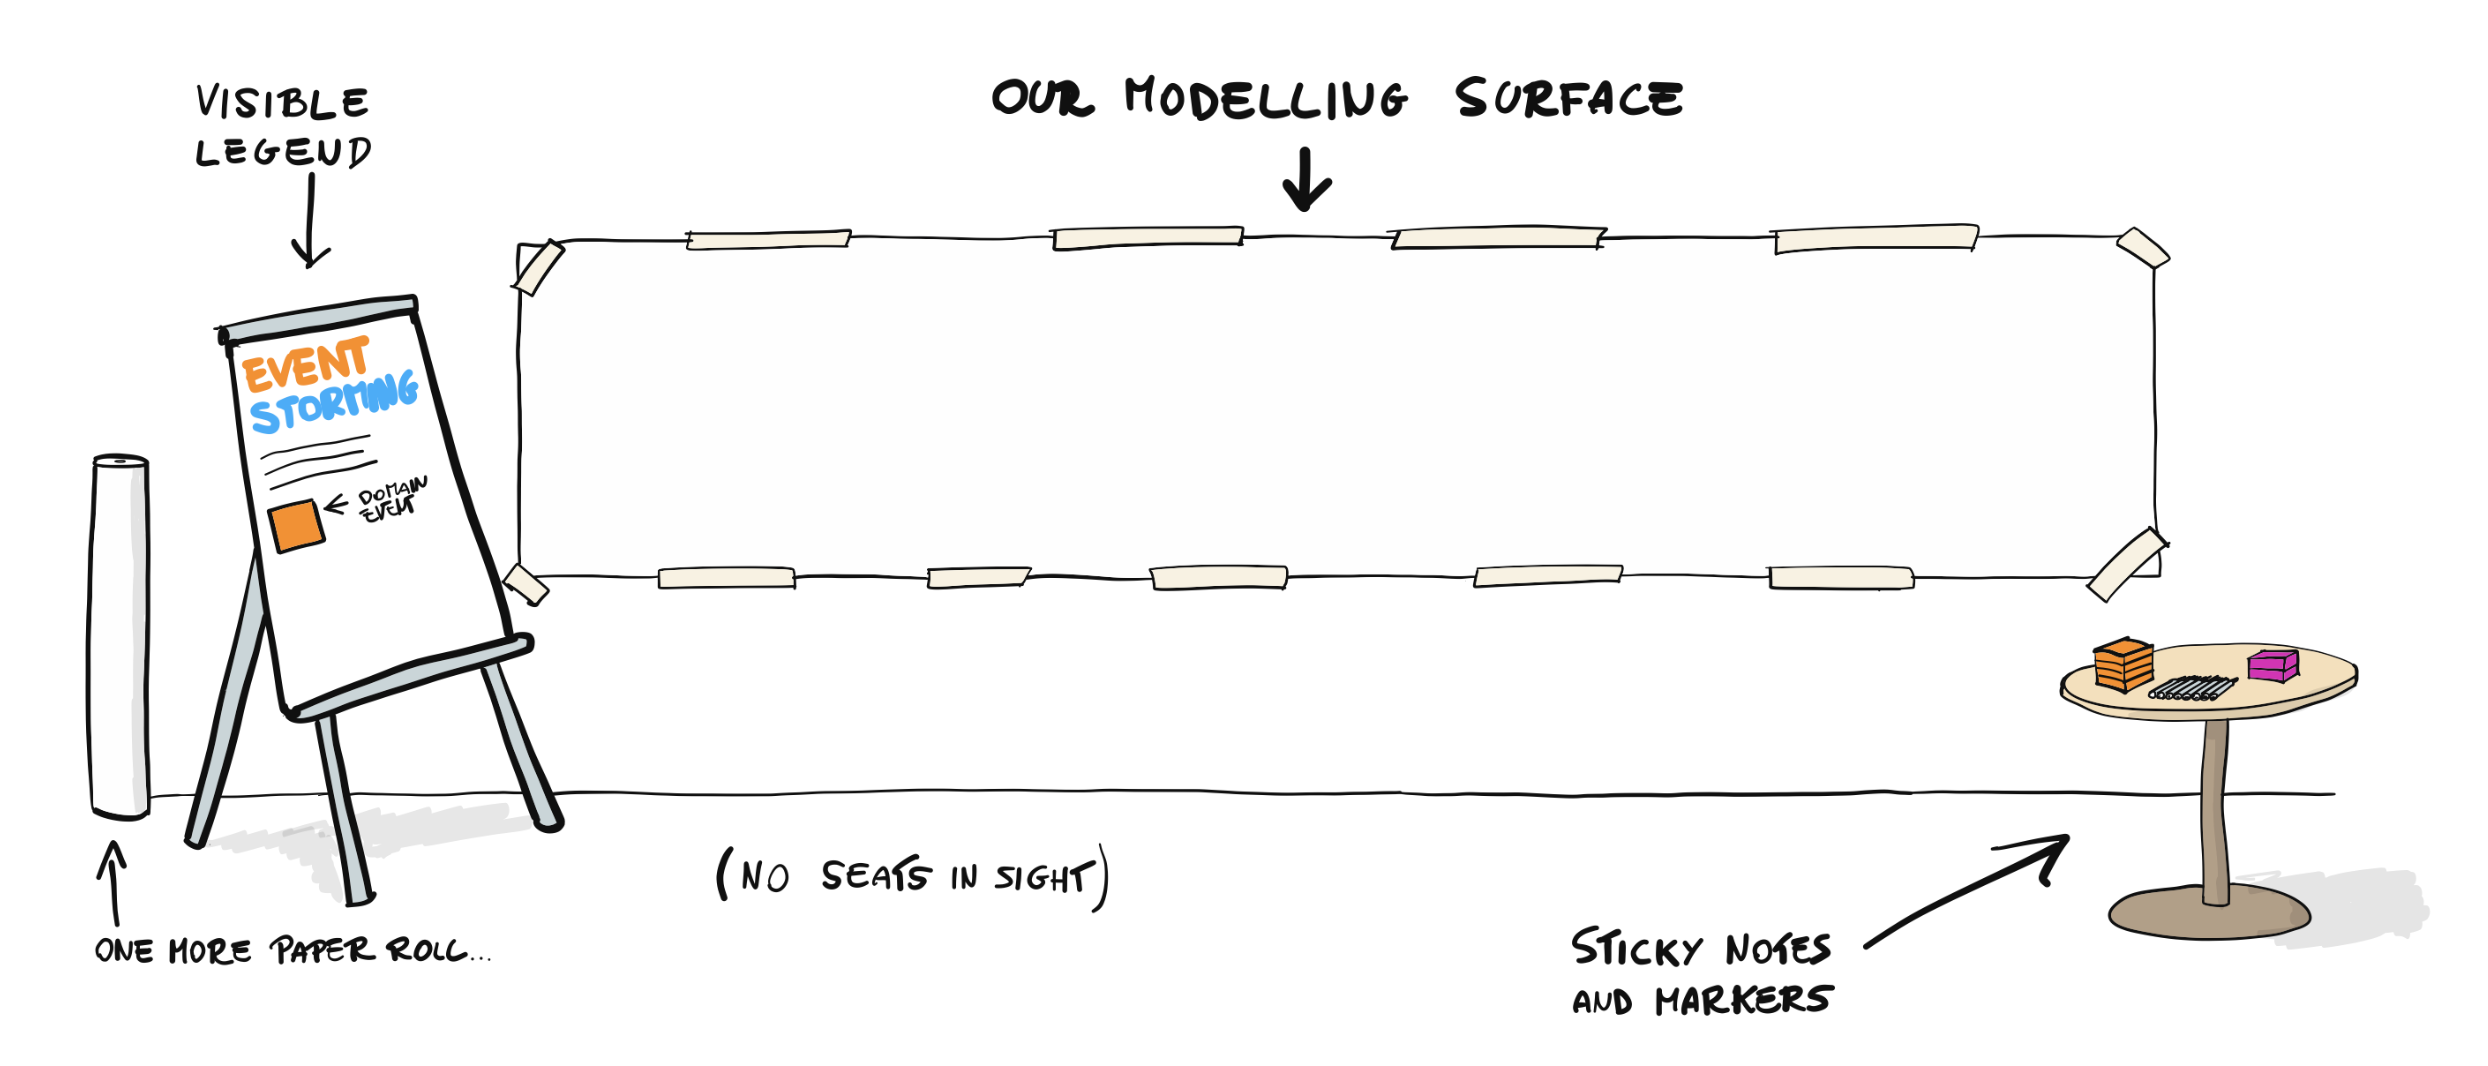
\includegraphics[width=0.8\textwidth]{images/event-storming-setup.png}
  \caption{Preparazione per una sessione di Event Storming}
  \label{fig:event-storming-setup}
\end{figure}

\subsubsection{Svolgimento della riunione}
\label{sec:svolgimento-della-riunione}
Intorno alle 9:30 è iniziata la riunione; si poteva notare che i partecipanti erano spaesati ma allo stesso tempo incuriositi dal grande rotolo di carta. 
Linda, nel ruolo di facilitatore, ha lanciato il meeting con un breve giro di presentazioni.
Successivamente, ha spiegato in maniera esplicita l'obiettivo della riunione in modo che fosse chiaro a tutti i partecipanti.
\\

\begin{tabularx}{.9\textwidth}{rX}
\speak{Linda} & L'obiettivo di questo incontro è analizzare gli attuali processi aziendali del caseificio per cercare di capire come possano essere migliorati e automatizzati interagendo armonicamente fra loro e con sistemi preesistenti. All'inizio il processo potrebbe sembrarvi difficile ma vi invito a intervenire senza paura, qualunque cosa facciate sarà utile.
\end{tabularx}
\\

La spiegazione del facilitatore è volutamente molto breve: non si vuole annoiare con una lunga descrizione ma lasciare che gli esperti di dominio inizino subito a descrivere il loro lavoro. L'importante è che il facilitatore trasmetta una sensazione di sicurezza e disponibilità ad aiutare i partecipanti.
\\

\begin{tabularx}{.9\textwidth}{rX}
  \speak{Linda} & Vorrei che descriveste degli eventi rilevanti al vostro ambito aziendale su questi post-it arancioni e che li mettiate in ordine cronologico su questo rotolo di carta. \\
  \speak{Raffaella} & Potresti spiegare meglio cosa intendete con ``eventi''? \\
  \speak{Linda} & Certamente! Ti faccio un esempio concreto: lavoro nel settore degli ordini, un evento che mi interessa è quando ricevo via email un nuovo ordine\\
  & \emph{Mentre parla, Linda scrive la frase ``Nuovo ordine ricevuto per email'' su un post-it arancione}\\
  \speak{Raffaella} & Ah, adesso mi è chiaro... quindi un evento che mi interessa potrebbe essere ``Fatto nuovo piano di produzione''?\\
  \speak{Linda} & Esatto! L'importante è che nel descrivere l'evento usiate sempre un verbo al passato come ha fatto Raffaella 
\end{tabularx}

\todo[inline]{Mettere il video}
